\documentclass[10pt]{article}
\usepackage{ctex}
\usepackage{graphicx}
\graphicspath{{E:/大学课程/大一下/人工智能程序设计/作业集/第三次作业/},{pics/}}
\usepackage{amsmath}
\usepackage{amssymb}
\usepackage{float}%使图片紧跟在文字后面

\title{第三周平时作业}
\author{朱士杭\ 231300027}
\date{\kaishu \today}

\begin{document}
	\maketitle
\section{python中if-elif-else语句工作原理}
	条件分支语,先判断if语句条件表达式是否成立是True还是False,并且满足短路求值,即一旦前面部分的表达式已经决定了整个条件表达式的True或者False的时候就不再继续求表达式的值了;如果if满足则执行if下面的语句,执行完以后跳出,不再执行elif与else;如果if不满足则执行elif下面的雨具,执行完以后跳出,不再执行else语句;如果if与elif条件表达式都不满足,则执行else下的语句
\section{while循环}
	while循环主要用于判断事件的循环\par
	这里需要一个计数器i=2每执行完一次while循环计数器都需要+2
	\begin{figure}[H]
		\centering
		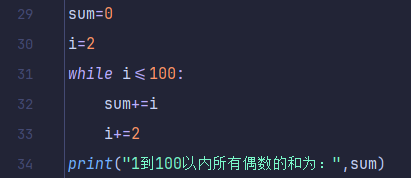
\includegraphics[scale=1]{2到100以内所有偶数之和}
		\caption{2到100以内所有偶数之和}
	\end{figure}
\section{迭代器与生成器}
	\subsection{迭代器}
	迭代器主要是对于一个可迭代对象进行遍历的一个工具,相当于一个指针指向这个可迭代对象,使用iter()函数获取该迭代器,通过next()函数获取迭代器下一个所指向的元素,并且将迭代器自动向下一个元素移动,直到移动到可迭代对象最后一个元素为止。\par
	迭代器使用过一次就相当于失效了,需要生成一个新的迭代器\par
	下图中由于已经遍历完整个迭代器对象,迭代器已经失效,再使用next()函数则会报错
	\begin{figure}[H]
		\centering
		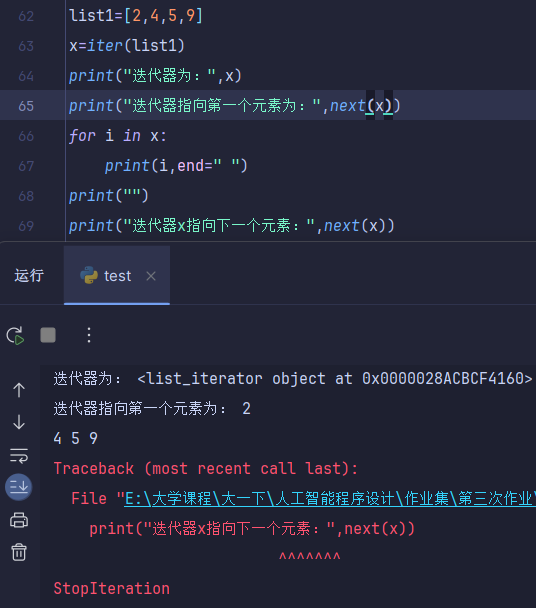
\includegraphics[scale=0.9]{迭代器}
		\caption{迭代器}
	\end{figure}
	\subsection{生成器}
	生成器相当于一个更加优雅的迭代器,在函数中通过与yield关键词语句搭配可以直接return内容的迭代器,当需要迭代器里面的元素的时候直接从yield下一行语句开始执行;而在列表解析的时候可以将[]替换为()从而获取该生成器,用next()函数的时候与普通迭代器用法一致
	\begin{figure}[H]
		\centering
		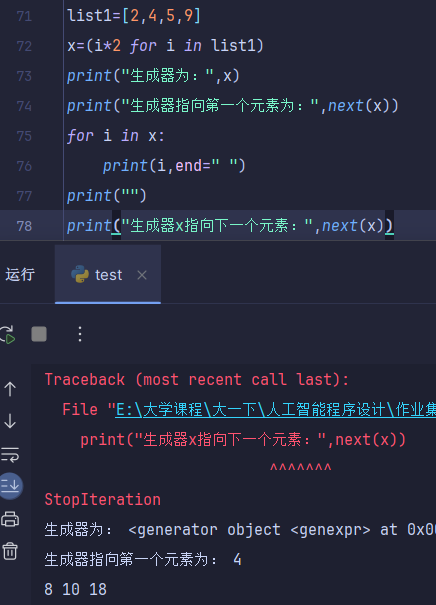
\includegraphics[scale=0.5]{生成器1}
		\caption{用()列表解析产生生成器}
	\end{figure}
		\begin{figure}[H]
		\centering
		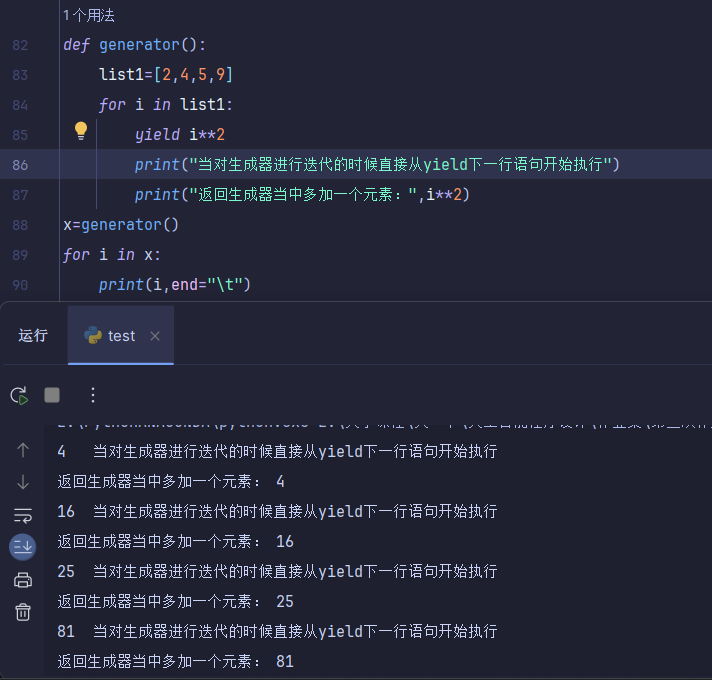
\includegraphics[scale=0.4]{生成器2}
		\caption{与yield关键字结合产生生成器}
	\end{figure}
\section{分析代码输出及其原因}	
	代码1:输出[1,4,9]  这里使用了列表解析的方式生成了一个列表\par
	代码2:输出[1,4,9]  这里用()生成了一个生成器对象squares,然后将该生成器进行强制类型转换成list列表。假如直接print(squares)则会输出$<generator object <genexpr> at 0x0000025737DC0BA0>$表明这是一个生成器对象
\section{条件表达式}
	返回一个bool值True或False类型的函数,相当于C++里面的:表达式?值1:值2 满足表达式返回值1,不满足返回值2
	\begin{figure}[H]
		\centering
		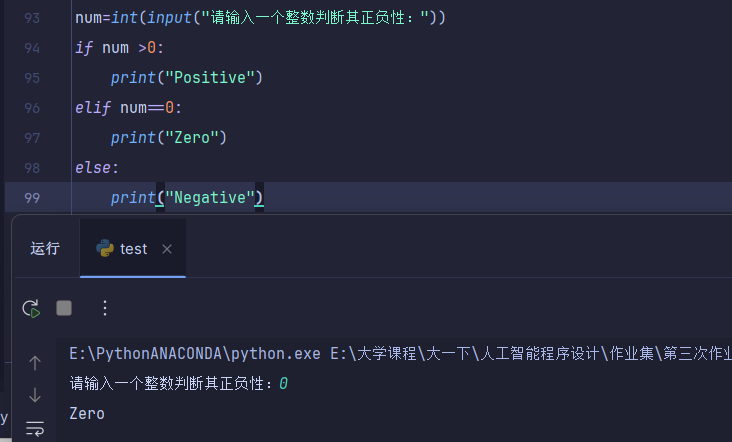
\includegraphics[scale=0.8]{正负}
		\caption{条件表达式判断正负}
	\end{figure}
\section{文件读写}
	\begin{figure}[H]
		\centering
		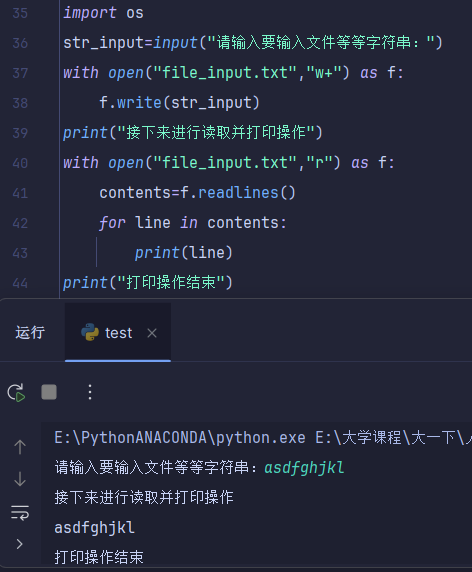
\includegraphics[scale=1]{文件读写}
		\caption{文件写入字符串并读取打印}
	\end{figure}
\end{document}